\documentclass[../main.tex]{subfiles}
\begin{document}
\chapter{First-Order Differential Equations}
\begin{remark}[Terminology]
  \begin{itemize}
    \item \textbf{n-th order - } Differential equation where the \textbf{highest} order derivative is $n$.
    \item \textbf{Linear -} Dependant variable and its derivatives only appear linearly.
    \item \textbf{Ordinary (ODE) -} Involves a function of one variable.
  \end{itemize}
  \begin{example}
    For example, $x^2y + y' = 0$ is a first order linear ODE.
  \end{example}
\end{remark}
\section{Exponential Function}
\begin{definition}[Exponential Function]
  The \textit{exponential function} is defined by the infinite series:
  \[
    \exp(x) = \sum_{n=0}^{\infty} \frac{x^{n}}{n!} = 1 + x + \frac{x^2}{2!} + \frac{x^3}{3!} + \cdots
  \]
\end{definition}
This can also be written as a limit:
\begin{align*}
  \exp(x) &= \lim_{k \to \infty} \left(1 + \frac{x}{k}\right)^{k} \\
          &= \lim_{k \to \infty} \left[1 + k\left(\frac{x}{k}\right) + \frac{k(k-1)}{2!}\left(\frac{x}{k}\right)^2 + \cdots\right] \text{ (Using binomial theorem)}\\
          &= 1 + x + \frac{x^2}{2!} + \frac{x^3}{3!} + \cdots
\end{align*}
If we differentiate the series we get:
\begin{align*}
  \deriv{}{x}\exp(x) &= 1 + \frac{2}{2!} x + \frac{3}{3!} x^2 + \cdots \\
                     &= 1 + x + \frac{x^2}{2!} + \frac{x^3}{3!} + \cdots \\
                     &= \exp(x)
\end{align*}
We can also define the exponential function to be the solution of the ODE:
\[
  \deriv{f}{x} = f \text{ with }f(0) = 1
\]
The exponential function also has the following key property:
\[
  \exp(x_1)\exp(x_2) = \exp(x_1 + x_2)
\]
This means acts similarly to exponentiation so we write $\exp(x) = e^{x}$ where:
\[
  e = \exp(1) = \lim_{k \to \infty} \left(1 + \frac{1}{k}\right)^{k}
\]
The inverse function of the exponential function is the natural logarithm, $\ln x$ or $\log_{e} x$, where $\exp(\ln x) = x$.
It follows that $a^{x} = (e^{\ln a})^{x} = e^{x \ln a}$ and thus $\deriv{}{x}a^{x} = \ln a e^{x \ln a} = a^{x} \ln a$.
\begin{definition}[Eigenfunction]
  An \textit{eigenfunction} of the derivative operator is is a function that is unchanged up to multiplicative scaling by the \textit{eigenvalue}, under the action of the operator.
  That is:
  \[
    \deriv{}{x}f(x) = \lambda f(x)
  \]
  where $\lambda$ is the \textit{eigenvalue}.
\end{definition}
From the properties we discussed earlier we can see that $e^{\lambda x}$ is an eigenfunction of the derivative operator.
\section{First Order Linear ODEs}
\begin{remark}
  Any $n$-th order linear ODE has $n$ independent solutions.
\end{remark}
\begin{definition}[Homogeneous]
  A \textit{homogeneous} ODE is one in which all terms involve the dependant variable or its derivatives.
\end{definition}
This means that $y = 0$ is always a solution of a homogeneous ODE.
This is called the ``trivial solution''.
\begin{remark}
  For any linear homogeneous ODE, any constant multiple of a solution is also a solution.
\end{remark}
\subsection{Homogeneous Linear ODEs with Constant Coefficients}
\begin{definition}[Constant Coefficients]
  A differential equation has \textit{constant coefficients} if the independent variable does not appear explicitly.
\end{definition}

Solutions of linear homogeneous ODEs with constant coefficients (for any order) are of the form $e^{\lambda x}$ (i.e. $x^{n}e^{\lambda x}$ and linear combinations of these).
\begin{example}
  \[
    5\deriv{y}{x} - 3y = 0
  \]
  Try a solution of the form $y = Ae^{\lambda x}$.
  \begin{align*}
    5\lambda Ae^{\lambda x} - 3Ae^{\lambda x} &= 0 \\
    Ae^{\lambda x}(5\lambda - 3) &= 0
  \end{align*}
  $A= 0$ gives the trivial solution so for non-trivial solutions we must have $5\lambda - 3 = 0$.
  This is called the ``characteristic equation''.
  \[
    \lambda = \frac{3}{5} \implies y = Ae^{\frac{3x}{5}}
  \]
  This is called the ``general solution''.
  To specify a unique solution requires us to apply suitable boundary condition(s).
  In general, we need $n$ boundary conditions to get a unique solution for an $n$-th order ODE.

  For example if we had the boundary condition $y(0) = y_0$ then $A = y_0$ so the solution is $y = y_0 e^{3x/5}$.
\end{example}

\subsection{Discrete Equations}
It is sometimes useful to consider a function evaluated at discrete points.
\begin{example}
  Consider again $5y' - 3y = 0$, $y(0) = y_0$.
  We can then approximate the equation by a discrete form at some set of points $\{x_n\}$ with $x_n = nh$ with $x_0 = 0$.

  One way we can approximate the derivative is with the ``Forward Euler Scheme'':
  \[
    \at{\deriv{y}{x}}{x_n} \approx \frac{y_{n+1} - y_n}{h}
  \]
  This is not a great approximation but is sufficient for this example.
  \begin{center}
  \begin{tikzpicture}[scale=1.2]
    \draw[->] (0, 0) -- (6.5, 0) node[right] {$x$};
    \draw[->] (0, 0) -- (0, 5.3) node[above] {$y$};

    \def\h{1}
    \def\yzero{0.26}
    \def\nsteps{6}

    \coordinate (P0) at (0,\yzero);
    \fill (P0) circle (1pt);
    \node[left] at (P0) {\small$y_0$};
    \node[below] at (0, 0) {$x_0$};

    \pgfmathsetmacro{\x}{0}
    \pgfmathsetmacro{\y}{\yzero}

    \foreach \i in {1,...,\nsteps} {
      \pgfmathsetmacro{\f}{0.5*\y}
      \pgfmathsetmacro{\ynew}{\y + \h*\f}
      \pgfmathsetmacro{\xnew}{\x + \h}

      \draw (\x,\y) -- (\xnew,\ynew);
      \draw[dashed] (\xnew, \ynew) -- (\xnew, 0);
      \node[below] at (\xnew, 0) {$x_\i$};
      \node[below right] at (\xnew, \ynew) {\small$y_\i$};

      \fill (\xnew,\ynew) circle (1pt);

      \xdef\y{\ynew}
      \xdef\x{\xnew}
    }

    \draw[thick, domain=0:6, smooth, samples=100] plot (\x,{\yzero * exp(0.5*\x)});
  \end{tikzpicture}
  \end{center}
  Substituting this back into the original DE yields:
  \begin{align*}
    5\left(\frac{y_{n+1}-y_n}{h}\right) - 3y_n &= 0 \\
    y_{n+1} &= \left(1 + \frac{3}{5}h\right)y_n
  \end{align*}
  This is a \textit{recurrence relation} for $y_n$.
  \begin{align*}
    y_n &= \left(1 + \frac{3}{5}h\right)y_{n-1} = \left(1 + \frac{3}{5}h\right)^2 y_{n - 2} = \cdots \\
        &= \left(1 + \frac{3}{5}h\right)^{n}y_0 = \left(1 + \frac{3x_n}{5n}\right)^{n}y_0
  \end{align*}
  Now take $x_n = x$ ($n$ steps from $x = 0$ to $x$) as $n \to \infty$:
  \[
    y(x) = \lim_{n \to \infty} y_n = \lim_{n \to \infty} y_0 \left(1 + \frac{3x}{5n}\right)^{n} = y_0 \exp\left(\frac{3x}{5}\right)
  \]
  which agrees with the continuous case.
\end{example}
\subsection{Series Solutions}
Series solutions are a powerful way to solve ODEs.
This involves looking for a solution in the form of a power series:
\[
  y(x) = \sum_{n=0}^{\infty} a_n x^{n}
\]
We can then determine the coefficients $a_n$ by substituting into the ODE.
\begin{example}
  Again using $5y' - 3y = 0$.
  \[
    \deriv{y}{x} = \sum_{n=0}^{\infty} na_n x^{n-1} = \sum_{n=1}^{\infty} na_nx^{n-1}
  \]
  For convenience consider:
  \[
    x \deriv{y}{x} = \sum_{n=1}^{\infty} na_n x^{n}
  \]
  Moreover:
  \[
    xy = \sum_{n=0}^{\infty} a_n x^{n + 1} = \sum_{m = 1}^{\infty} a_{m-1}x^{m} = \sum_{n = 1}^{\infty} a_{n-1}x^{n}
  \]
  We can then substitute into the ODE multiplied by $x$:
  \begin{align*}
    5xy' - 3xy &= 0 \\
    \sum_{n=1}^{\infty} (5na_n - 3a_{n-1})x^{n} &= 0 \\
  \end{align*}
  This is true for all $x$ so $5na_n -3a_{n-1}$ must be zero for all $n\geq1$.
  Thus:
  \begin{align*}
    a_n &= \frac{5}{3n}a_{n-1},\ n\geq1 \\
        &= \frac{5}{3n}\frac{5}{3(n-1)}a_{n-2} \\
        &\;\;\vdots \\
        &= \left(\frac{3}{5}\right)^{n} \frac{1}{n!}a_0
  \end{align*}
  so:
  \[
    y(x) = a_0 \sum_{n=0}^{\infty} \frac{1}{n!}\left(\frac{3x}{5}\right)^{n} = a_0 \exp\left(\frac{3x}{5}\right)
  \]
  which agrees with the other methods.
\end{example}
\section{Forced ODEs}
\begin{definition}[Forced]
  A \textit{forced} ODE is one which includes terms that \textbf{do not} include the dependant variable or its derivatives.
  This is the same as it being \textit{non-homogeneous} or \textit{inhomogeneous}.
\end{definition}
\begin{remark}
  In general, $y = 0$ is \textbf{not} a solution to forced ODEs.
\end{remark}
\subsubsection{Method To Solved Forced ODEs}
\begin{enumerate}
  \item Find \textbf{any} solution of the forced equation.
        This gives you a particular integral (P.I.), $y_p(x)$.
  \item Write general solution as $y(x) = y_p(x) + y_c(x)$ and find complimentary function (C.F.), $y_c(x)$, that satisfies the corresponding homogeneous equation.
  \item Combine $y_p$ and $y_c$ to get general solution.
\end{enumerate}
\begin{remark}[Warning]
  This only works for \textbf{linear} forced ODEs otherwise the superposition of two solutions is not always a solution.
\end{remark}
\subsection{Constant Forcing}
\begin{example}
  Consider $5y' - 3y = 10$.
  10 is called the ``constant forcing term''.

  We first guess that $y_p(x)$ is a constant, thus $y_p(x) = - \frac{10}{3}$.
  $y_c(x) = Ae^{\frac{3x}{5}}$ is the solution of the homogeneous equation ($5y' - 3y = 0$).
  So the general solution is:
  \[
    y(x) = Ae^{\frac{3x}{5}} - \frac{10}{3}
  \]
\end{example}
\subsection{Eigenfunctfion Forcing}
In eigenfunction forcing, the forcing term is an eigenfunction of the differential operator.
\begin{example}[Radioactive Decay]
  Suppose we have three isotopes $A$, $B$, $C$ where:
  \[
    \underbrace{A}_{a(t)} \xrightarrow{k_a a} \underbrace{B}_{b(t)} \xrightarrow{k_b b} \underbrace{C}_{c(t)}
  \]
  Isotope only decays out of A so:
  \[
    \deriv{a}{t} = -k_a a \implies a = a_0 e^{-k_a t}
  \]
  We can now form a differential equation for $b$:
  \begin{align*}
    \deriv{b}{t} &= k_a a -k_b b \\
    \deriv{b}{t} + k_b b &= \underbrace{k_a a_0 e^{-k_a t}}_{\text{forcing}} \\
    \label{radioactive}
  \end{align*}
  Try a P.I., $b_p(t) = \beta e^{-k_a t}$:
  \begin{align*}
    (k_b - k_a)\beta e^{-k_a t} &= k_a a_0e^{-k_a t} \\
    \implies \beta &= \frac{k_a a_0}{k_b - k_a}\quad(k_a \neq k_b)
  \end{align*}
  $b_c(t)$ solves $b_c' + k_b b_c = 0$ so $b_c(t) = De^{-k_b t}$.
  So the general solution is:
  \[
    b(t) = De^{-k_b t} + \frac{k_a}{k_b - k_a}a_0 e^{-k_a t}
  \]
  Now suppose we have $b(0) = 0$ so:
  \[
    b(t) = \frac{k_a a_0}{k_b - k_a}(e^{-k_a t} - e^{-k_b t})
  \]
  \begin{center}
  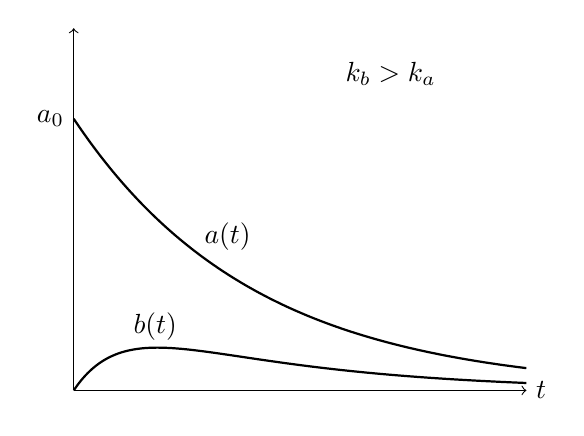
\begin{tikzpicture}[scale=1.15]
    \draw[->] (0, 0) -- (5, 0) node[right] {$t$};
    \draw[->] (0, 0) -- (0, 4);

    \def\ka{0.5}
    \def\azero{3}
    \def\kb{2}
    \node[left] at (0, \azero) {$a_0$};

    \node at (1.7, 1.7) {$a(t)$};
    \node at (0.9, 0.7) {$b(t)$};
    \node at (3.5, 3.5) {$k_b > k_a$};

    \draw[thick, domain=0:5, smooth, samples=100] plot (\x,{\azero * exp(-\ka*\x)});
    \draw[thick, domain=0:5, smooth, samples=100] plot (\x,{((\ka * \azero)/(\kb - \ka)) * (exp(-\ka*\x) - exp(-\kb*\x)});
  \end{tikzpicture}
  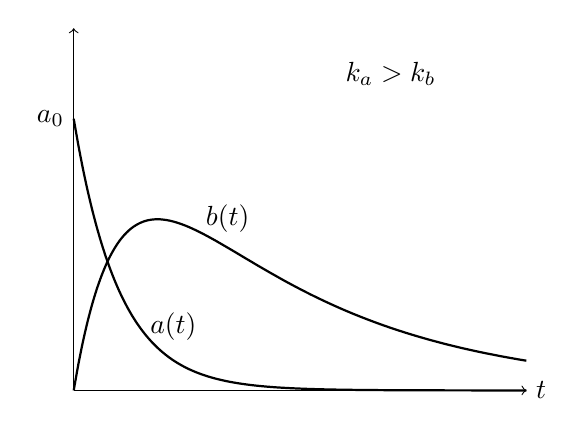
\begin{tikzpicture}[scale=1.15]
    \draw[->] (0, 0) -- (5, 0) node[right] {$t$};
    \draw[->] (0, 0) -- (0, 4);

    \def\ka{2}
    \def\azero{3}
    \def\kb{0.5}
    \node[left] at (0, \azero) {$a_0$};

    \node at (1.7, 1.9) {$b(t)$};
    \node at (1.1, 0.7) {$a(t)$};
    \node at (3.5, 3.5) {$k_a > k_b$};

    \draw[thick, domain=0:5, smooth, samples=100] plot (\x,{\azero * exp(-\ka*\x)});
    \draw[thick, domain=0:5, smooth, samples=100] plot (\x,{((\ka * \azero)/(\kb - \ka)) * (exp(-\ka*\x) - exp(-\kb*\x)});
  \end{tikzpicture}
  \end{center}
  If $k_a = k_b$, we need a different P.I., this will be discussed later in \cref{differentPI}.
\end{example}
\section{Non-Constant Coefficients}
The general form of a first order linear ODE with \textit{non-constant coefficients}, that is, the independent variable appears explicitly, is:
\[
  a(x)\deriv{y}{x} + b(x)y = c(x)
\]
or the ``standard-form'':
\[
  \deriv{y}{x} + p(x)y = f(x)
\]
We can solve these using an \textit{integrating factor} (I.F.), $\mu(x)$.

Start by multiplying the ODE by $\mu$:
\[
  \mu y' + \mu py = \mu f
\]
We want the left hand side to be equal to $(\mu y)' = \mu y' + \mu' y$.
This is true if $\mu' = \mu p$.
So we require that
\[
  \frac{\mu'}{\mu} = p \implies \int p \d{x} = \int \frac{\mu'}{\mu} \d{x} = \ln \mu \quad\text{(Up to a constant)}
\]
Thus:
\[
  \mu(x) = \exp\left[\int^x P(u) \d{u}\right]
\]
which is unique up to an irrelevant constant factor as this multiple would just cancel out on either side of the DE as it is linear.
\[
  \deriv{}{x}(\mu y) = \mu f \implies \mu y = \int^x \mu(u)f(u) \d{u}
\]
\begin{example}
  Consider $xy' + (1-x)y = 1$.
  First convert to standard form:
  \[
    y' + \underbrace{\frac{1-x}{x}}_{p(x)}y = \underbrace{\frac{1}{x}}_{f(x)}
  \]
  So the I.F. is:
  \begin{align*}
    \ln \mu &= \int_{}^{x} \left(\frac{1}{u} - 1\right) \d{u} \\
            &= \ln x - x \\
            &= \ln(xe^{-x}) \\
    \mu &= xe^{-x}
  \end{align*}
  Therefore:
  \begin{align*}
    \deriv{}{x}(xe^{-x}y) &= \frac{x}{x}e^{-x} = e^{-x}\\
    xe^{-x}y &=-e^{-x} + C \\
    y &= -\frac{1}{x} + \frac{C}{x}e^{x}
  \end{align*}
  Note that we could set $C=1$ if we want finite $y$ as $x \to 0$.
\end{example}
\begin{example}[Radioactive Decay Revisited]
  Recall from \cref{radioactive} we had:
  \[
    \deriv{b}{t} + \underbrace{k_b}_{p(t)}b = \underbrace{k_a a_0 e^{-k_a t}}_{f(t)}
  \]
  So the I.F. is $\mu = \exp(\int k_b \d{t}) = e^{k_b t}$ and so:
  \[
    \deriv{}{t}(e^{k_b t}b) = k_a a_0 e^{(k_b - k_a)t}
  \]
  \begin{proofcases}
    \begin{case}{$k_b \neq k_a$}
      \begin{align*}
        e^{k_b t}b &= \frac{k_0 a_0}{k_b - k_a}e^{(k_b - k_a)t} +C \\
              b(t) &= \underbrace{\frac{k_0 a_0}{k_b - k_a}e^{-k_a t}}_{\text{P.I.}} + \underbrace{Ce^{-k_b t}}_{\text{C.F.}}
      \end{align*}
      Which agrees with what we had earlier.
    \end{case}
    \label{differentPI}
    \begin{case}{$k_a = k_b$}
      So the right hand side is just $k_a a_0$ which is independent of $t$ so:
      \begin{align*}
        e^{k_b t}b &= k_a a_0 t + C \\
        b(t) &= \underbrace{k_a a_0 t e^{-k_b t}}_{\text{P.I.}} + \underbrace{Ce^{-k_b t}}_{\text{C.F.}}
      \end{align*}
      So $\text{P.I.} \propto t e^{-k_b t}$ not just $e^{-k_b t}$, so if we tried $\beta t e^{-k_b t}$ earlier we would have gotten this result.
      \begin{center}
      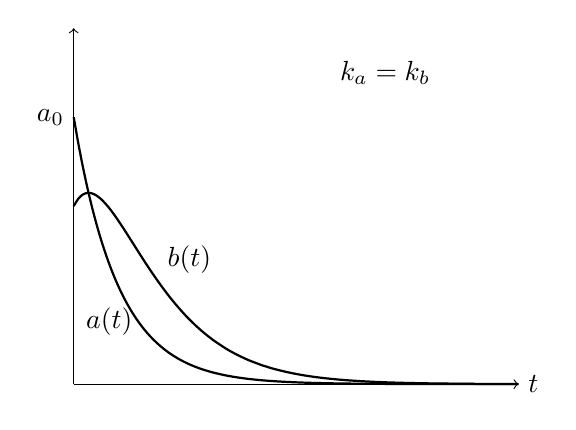
\begin{tikzpicture}[scale=1.13]
        \draw[->] (0, 0) -- (5, 0) node[right] {$t$};
        \draw[->] (0, 0) -- (0, 4);

        \def\kab{2}
        \def\azero{3}
        \node[left] at (0, \azero) {$a_0$};

        \node at (1.3, 1.4) {$b(t)$};
        \node at (0.4, 0.7) {$a(t)$};
        \node at (3.5, 3.5) {$k_a = k_b$};

        \draw[thick, domain=0:5, smooth, samples=100] plot (\x,{\azero * exp(-\kab*\x)});
        \draw[thick, domain=0:5, smooth, samples=100] plot (\x,{(\kab * \azero * \x + 2)* exp(-\kab * \x))});
      \end{tikzpicture}
      \end{center}
    \end{case}
  \end{proofcases}
\end{example}

\section{Non-Linear First-Order ODEs}
Non-linear first-order ODEs have the general form:
\begin{equation}
  \label{nonLinearGeneral}
  Q(x, y)\deriv{y}{x} + P(x, y) = 0
\end{equation}
\begin{remark}
  These could be non-linear in $\deriv{y}{x}$ too but we are not considering those within this course.
\end{remark}
\subsection{Separable Equations}
A first order ODE is \textit{separable} if it can be written as:
\[
  Q(y) \d{y} = P(x) \d{x}
\]
We can solve these by direct integration:
\[
  \int Q(y) \d{y} = \int P(x) \d{x}
\]
\begin{example}
  Consider the differential equation:
  \begin{align*}
    (x^2y - 3y)\deriv{y}{x} - 2xy^2 &= 4x \\
    y(x^2 - 3)\deriv{y}{x} &= 2x(2 + y^2) \\
    \frac{y}{2 + y^2} \d{y} &= \frac{2x}{x^2 -3} \d{x} \\
    \int \frac{y}{2 + y^2} \d{y} &= \int \frac{2x}{x^2 - 3} \d{x} \\
    \frac{1}{2}\ln(2 + y^2) &= \ln|x^2 - 3| + C \\
    \sqrt{y^2 + 2} &= A|x^2 - 3|
  \end{align*}
\end{example}
\subsection{Exact Equations}
\begin{definition}[Exact]
  A non-linear first order ODE is \textit{exact} if:
  \[
    P(x, y)\d{x} + Q(x, y)\d{y}
  \]
  is an \textit{exact differential}.
  That is, there exists a function, $f(x, y)$, such that:
  \[
    \d{f} = P(x, y)\d{x} + Q(x, y)\d{y}
  \]
\end{definition}
If \cref{nonLinearGeneral} is exact then $\d{f} = 0$ so $f(x, y) = \text{constant}$ is a solution.
We can use the multivariate chain rule (\cref{multiChainRule}) to get:
\[
  \d{f} = \underbrace{\pderiv{f}{x}}_{P(x, y)} \d{x} + \underbrace{\pderiv{f}{y}}_{Q(x, y)} \d{y}
\]
So we need to solve $\pderiv{f}{x} = P$ and $\pderiv{f}{y} = Q$.
We know that partial derivatives commute so:
\[
  \pderiv{P}{y} = \frac{\partial^2 f}{\partial y \partial x} = \frac{\partial^2 f}{\partial x \partial y} = \pderiv{Q}{x}
\]
Therefore, a \textit{necessary} but not sufficient condition for the ODE to be exact is:
\[
  \pderiv{P}{y} = \pderiv{Q}{x}
\]
\begin{theorem}
  If $\pderiv{P}{y} = \pderiv{Q}{x}$ throughout a simply connected domain $\mathcal{D}$, $P\d{x} + Q\d{y}$ is an exact differential of a single-valued function $f(x, y)$ in $\mathcal{D}$.
\end{theorem}
\begin{definition}[Simply Connected]
  A domain $\mathcal{D}$ is \textit{simply connected} if it is path connected and any closed curve in $\mathcal{D}$ can be continuously shrunk to a point in $\mathcal{D}$ without leaving $\mathcal{D}$.
\end{definition}
\begin{definition}[Path Connected]
  A domain $\mathcal{D}$  is \textit{path connected} if every pair of points in $\mathcal{D}$ can be connected by a path in $\mathcal{D}$.
\end{definition}
\begin{example}
Here are some examples of some path connected and simply connected domains:
\begin{center}
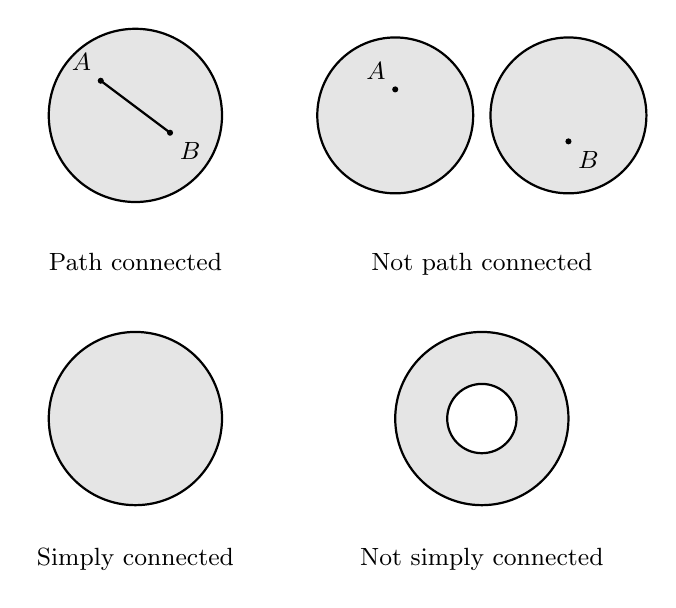
\begin{tikzpicture}[scale=1.1, every node/.style={font=\small}]
  \def\xshiftleft{-2cm}
  \def\xshiftright{2cm}
  \def\yshiftbottom{-3.5cm}

  \begin{scope}[xshift=\xshiftleft]
    \filldraw[fill=gray!20, draw=black, thick] (0,0) circle (1);
    \fill (-0.4,0.4) circle (1pt) node[above left] {$A$};
    \fill (0.4,-0.2) circle (1pt) node[below right] {$B$};
    \draw[thick] (0.4,-0.2) -- (-0.4,0.4);
    \node[below,yshift=-0.2cm] at (0,-1.3) {Path connected};
  \end{scope}

  \begin{scope}[xshift=\xshiftright]
    \filldraw[fill=gray!20, draw=black, thick] (-1,0) circle (0.9);
    \filldraw[fill=gray!20, draw=black, thick] (1,0) circle (0.9);
    \fill (-1,0.3) circle (1pt) node[above left] {$A$};
    \fill (1,-0.3) circle (1pt) node[below right] {$B$};
    \node[below,yshift=-0.2cm] at (0,-1.3) {Not path connected};
  \end{scope}

  \begin{scope}[yshift=\yshiftbottom, xshift=\xshiftleft]
    \filldraw[fill=gray!20, draw=black, thick] (0,0) circle (1);
    \node[below,yshift=-0.2cm] at (0,-1.2) {Simply connected};
  \end{scope}

  \begin{scope}[yshift=\yshiftbottom, xshift=\xshiftright]
    \filldraw[fill=gray!20, draw=black, thick] (0,0) circle (1);
    \filldraw[fill=white, draw=black, thick] (0,0) circle (0.4);
    \node[below,yshift=-0.2cm] at (0,-1.2) {Not simply connected};
  \end{scope}
\end{tikzpicture}
\end{center}
\end{example}

\begin{example}
  Consider the first order non-linear ODE:
  \begin{align*}
    6y(y-x)\deriv{y}{x} + 2x - 3y^2 &= 0 \\
    \underbrace{(2x - 3y^2)}_{P}\d{x} + \underbrace{6y(y - x)}_{Q}\d{y} &= 0
  \end{align*}
  Therefore we have:
  \[
    \pderiv{P}{y} = -6y \text{ and } \pderiv{Q}{x} = -6y \implies \pderiv{P}{y} = \pderiv{Q}{x}
  \]
  So this is exact in any simply connected domain.
  \begin{align*}
    P = \at{\pderiv{f}{x}}{y} &= 2x - 3y^2 \\
    \implies f(x, y) &= \int 2x - 3y^2 \d{x} \\
                     &= x^2 - 3xy^2 + h(y)
  \end{align*}
  Note we have a constant of integration that is a function of $y$ as $\pderiv{}{x}h(y) = 0$.
  \[
    Q = \at{\pderiv{f}{y}}{x} = 6y^2 - 6xy
  \]
  But we can also get $\at{(\partial f)/(\partial y)}{x}$ by differentiating our current expression for $f(x, y)$ with respect to $y$:
  \begin{align*}
    \at{\pderiv{f}{y}}{x} &= \pderiv{}{y}(x^2 - 3xy^2 + h(y)) \\
                          &= -6xy + \deriv{h}{y}\\
  \end{align*}
  Equating the two expressions for $\at{(\partial f)/(\partial y)}{x}$ yields:
  \begin{align*}
    \deriv{h}{y} - 6xy &= 6y^2 - 6xy \\
    \deriv{h}{y} &= 6y^2 \\
    \implies h(y) &= 2y^3 + C
  \end{align*}
  Thus:
  \[
    f(x, y) = x^2 - 3xy^2 + 2y^3 + C
  \]
  Since $f(x, y)$ is a constant, the general solution of ODE is:
  \[
    x^2 - 3xy^2 + 2y^3 = A
  \]
\end{example}
\section{Solution Curves and Isoclines}
Non-linear ODEs are often impossible to solve in a simple closed form.
However we can analyse the behaviour of solutions with graphical methods.
\subsubsection{Solution Curves}
Consider $\deriv{y}{t} = f(t, y)$.
Each initial condition (e.g. $y(0) = y_0$) generates a distinct \textit{solution curve} or \textit{trajectory}.

For example with $y = y_0 e^{x}$:
\begin{center}
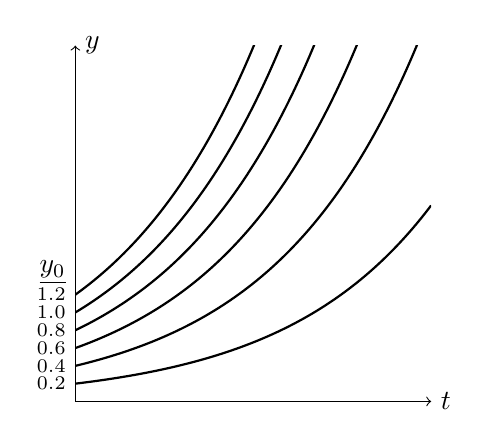
\begin{tikzpicture}[scale=1.13]
  \draw[->] (0, 0) -- (4, 0) node[right] {$t$};
  \draw[->] (0, 0) -- (0, 4) node[right] {$y$};


  \node[left] at (0, 1.45) {\underline{$y_0$}};
  \foreach \yzero in {0.2, 0.4, 0.6, 0.8, 1.0, 1.2}{
    \node[left] at (0, \yzero) {$\scriptstyle\yzero$};
    \begin{scope}
      \clip (0,0) rectangle (4, 4);
      \draw[thick, smooth, samples=100, domain=0:4] plot ({\x}, {\yzero * exp(0.6 * \x)});
    \end{scope}
  }
\end{tikzpicture}
\end{center}

This is useful as we can sketch the solution curve without needing to solve the ODE.
\begin{example}
  Consider the ODE:
  \[
    \deriv{y}{t} = t(1 - y^2)
  \]
  Note that this is separable so we can solve by direct integration:
  \begin{align*}
    \frac{\d{y}}{1 - y^2} &= t \d{t} \\
    \frac{1}{2}\left(\frac{1}{1+y} + \frac{1}{1-y}\right)\d{y} &= t\d{t} \\
    \frac{1}{2} \int \left(\frac{1}{1+y} + \frac{1}{1-y}\right) \d{y} &= \int t \d{t} \\
    \frac{1}{2}\ln \abs{\frac{1 + y}{1-y}} &= \frac{1}{2}t^2 + C \\
    \abs{\frac{1 + y}{1 - y}} &= e^{t^2} e^{2C}
  \end{align*}
  We now need to split into two cases depending on the value of $y$:
  \begin{proofcases}
    \begin{case}{$|y| < 1$}
      \vspace{-2em}
      \begin{align*}
        \frac{1 + y}{1 - y} &= e^{t^2} e^{2C} \\
        1 + y &= e^{t^2} e^{2C} - ye^{t^2} e^{2C} \\
        y(1 + e^{t^2}e^{2C}) &= e^{t^2} e^{2C} - 1 \\
        y(e^{-t^2} + e^{2C}) &= e^{2C} - e^{-t^2} \\
        y &= \frac{e^{2C} + e^{-t^2}}{e^{2C} - e^{-t^2}}
      \end{align*}
    \end{case}
    \begin{case}{$|y| > 1$}
      \vspace{-2em}
      \begin{align*}
        \frac{1 + y}{1 - y} &= - e^{t^2} e^{2C} \\
        1 + y &= ye^{t^2} e^{2C} - e^{t^2}e^{2C} \\
        y(e^{t^2}e^{2C} - 1) &= e^{t^2} e^{2C} + 1 \\
        y(-e^{2C} + e^{-t^2}) &= -e^{2C} - e^{-t^2} \\
        y &= \frac{-e^{2C} + e^{-t^2}}{-e^{2C} - e^{-t^2}}
      \end{align*}
    \end{case}
  \end{proofcases}
  So the general solution is:
  \[
    y = \frac{A - e^{-t^2}}{A + e^{-t^2}},\quad A = \begin{cases}
    e^{2C} & \text{ if } |y| < 1 \\
    -e^{-2C} & \text{ if } |y| > 1
    \end{cases}
  \]
  This means we have a family of solution curves parameterised by $A$.
  If $y(0) = y_0$ then $A = \frac{1 + y_0}{1 - y_0}$.
  \begin{center}
  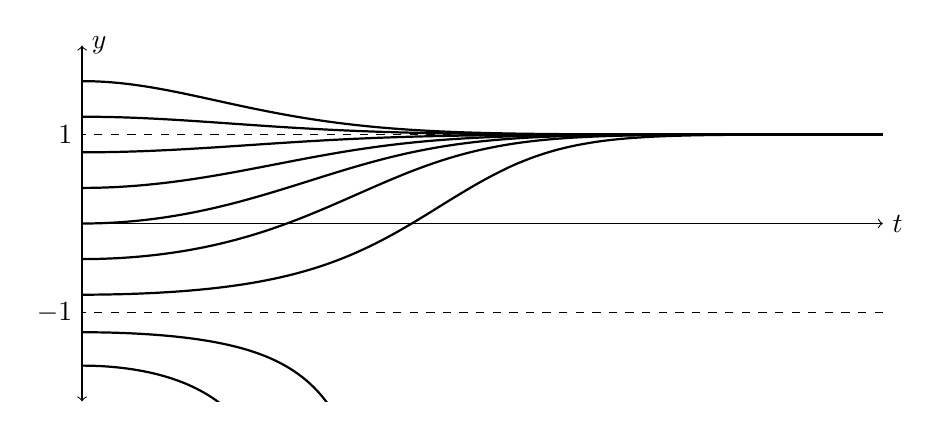
\begin{tikzpicture}[scale=1.13]
    \draw[->] (0, 0) -- (9, 0) node[right] {$t$};
    \draw[<->] (0, -2) -- (0, 2) node[right] {$y$};

    \draw[dashed] (9,1) -- (0, 1) node[left] {$1$};
    \draw[dashed] (9,-1) -- (0, -1) node[left] {$-1$};


    \clip (0,-2) rectangle (9,2);
    \foreach \yzero in {-0.8, -0.4, 0, 0.4, 0.8, 1.2, 1.6}{
      \pgfmathsetmacro{\Aconst}{(1+\yzero)/(1-\yzero)}
      \draw[thick, smooth, samples=100, domain=0:9] plot ({\x}, {(\Aconst - exp(-(0.4 * \x)^2))/(\Aconst + exp(-(0.4 * \x)^2))});
    }

    \draw[thick, smooth, samples=100, domain=0:3] plot ({\x}, {(-0.1 - exp(-(0.4 * \x)^2))/(-0.1 + exp(-(0.4 * \x)^2))});
    \draw[thick, smooth, samples=100, domain=0:3] plot ({\x}, {(-0.23 - exp(-(0.4 * \x)^2))/(-0.23 + exp(-(0.4 * \x)^2))});
  \end{tikzpicture}
  \end{center}
  Some properties of this are:
  \begin{itemize}
    \item For $-1 \leq A < 0$ we have a vertical asymptote.
    \item As $A \to -1$, $y_0 \to \infty$.
    \item As $A \to - \infty$, $y_0 \to 1^{+}$
    \item As $A \to \infty$, $y_0 \to 1^{-}$
    \item At $A = 0$ we have the constant solution $-1$.
    \item $y \to \pm 1$ as $t \to \infty$ for $A \neq 0$
  \end{itemize}

  We can also get some general behaviour directly from the ODE without needing to solve it:
  \begin{itemize}
    \item $\deriv{y}{t} = 0\ \forall t \text{ if } |y| = 1$.
      This means that we must have two constant solutions given by $y = \pm 1$.
    \item $\deriv{y}{t} = 0$ at $t = 0$ for all solutions.
  \end{itemize}
\end{example}
\end{document}
